\documentclass{article} % For LaTeX2e
\usepackage{iclr2024_conference,times}

\usepackage[utf8]{inputenc} % allow utf-8 input
\usepackage[T1]{fontenc}    % use 8-bit T1 fonts
\usepackage{hyperref}       % hyperlinks
\usepackage{url}            % simple URL typesetting
\usepackage{booktabs}       % professional-quality tables
\usepackage{amsfonts}       % blackboard math symbols
\usepackage{nicefrac}       % compact symbols for 1/2, etc.
\usepackage{microtype}      % microtypography
\usepackage{titletoc}

\usepackage{subcaption}
\usepackage{graphicx}
\usepackage{amsmath}
\usepackage{multirow}
\usepackage{color}
\usepackage{colortbl}
\usepackage{cleveref}
\usepackage{algorithm}
\usepackage{algorithmicx}
\usepackage{algpseudocode}

\DeclareMathOperator*{\argmin}{arg\,min}
\DeclareMathOperator*{\argmax}{arg\,max}

\graphicspath{{../}} % To reference your generated figures, see below.
\begin{filecontents}{references.bib}

@book{goodfellow2016deep,
  title={Deep learning},
  author={Goodfellow, Ian and Bengio, Yoshua and Courville, Aaron and Bengio, Yoshua},
  volume={1},
  year={2016},
  publisher={MIT Press}
}

@article{vaswani2017attention,
  title={Attention is all you need},
  author={Vaswani, Ashish and Shazeer, Noam and Parmar, Niki and Uszkoreit, Jakob and Jones, Llion and Gomez, Aidan N and Kaiser, {\L}ukasz and Polosukhin, Illia},
  journal={Advances in neural information processing systems},
  volume={30},
  year={2017}
}

@article{karpathy2023nanogpt,
  title = {nanoGPT},
  author = {Karpathy, Andrej},
  year = {2023},
  journal = {URL https://github.com/karpathy/nanoGPT/tree/master},
  note = {GitHub repository}
}

@article{kingma2014adam,
  title={Adam: A method for stochastic optimization},
  author={Kingma, Diederik P and Ba, Jimmy},
  journal={arXiv preprint arXiv:1412.6980},
  year={2014}
}

@article{ba2016layer,
  title={Layer normalization},
  author={Ba, Jimmy Lei and Kiros, Jamie Ryan and Hinton, Geoffrey E},
  journal={arXiv preprint arXiv:1607.06450},
  year={2016}
}

@article{loshchilov2017adamw,
  title={Decoupled weight decay regularization},
  author={Loshchilov, Ilya and Hutter, Frank},
  journal={arXiv preprint arXiv:1711.05101},
  year={2017}
}

@article{radford2019language,
  title={Language Models are Unsupervised Multitask Learners},
  author={Radford, Alec and Wu, Jeff and Child, Rewon and Luan, David and Amodei, Dario and Sutskever, Ilya},
  year={2019}
}

@article{bahdanau2014neural,
  title={Neural machine translation by jointly learning to align and translate},
  author={Bahdanau, Dzmitry and Cho, Kyunghyun and Bengio, Yoshua},
  journal={arXiv preprint arXiv:1409.0473},
  year={2014}
}

@article{paszke2019pytorch,
  title={Pytorch: An imperative style, high-performance deep learning library},
  author={Paszke, Adam and Gross, Sam and Massa, Francisco and Lerer, Adam and Bradbury, James and Chanan, Gregory and Killeen, Trevor and Lin, Zeming and Gimelshein, Natalia and Antiga, Luca and others},
  journal={Advances in neural information processing systems},
  volume={32},
  year={2019}
}

@misc{gpt4,
  title={GPT-4 Technical Report}, 
  author={OpenAI},
  year={2024},
  eprint={2303.08774},
  archivePrefix={arXiv},
  primaryClass={cs.CL},
  url={https://arxiv.org/abs/2303.08774}, 
}

@Article{Brown2020LanguageMA,
 author = {Tom B. Brown and Benjamin Mann and Nick Ryder and Melanie Subbiah and J. Kaplan and Prafulla Dhariwal and Arvind Neelakantan and Pranav Shyam and Girish Sastry and Amanda Askell and Sandhini Agarwal and Ariel Herbert-Voss and Gretchen Krueger and T. Henighan and R. Child and A. Ramesh and Daniel M. Ziegler and Jeff Wu and Clemens Winter and Christopher Hesse and Mark Chen and Eric Sigler and Ma-teusz Litwin and Scott Gray and B. Chess and Jack Clark and Christopher Berner and Sam McCandlish and Alec Radford and I. Sutskever and Dario Amodei},
 booktitle = {Neural Information Processing Systems},
 journal = {ArXiv},
 title = {Language Models are Few-Shot Learners},
 volume = {abs/2005.14165},
 year = {2020}
}

\end{filecontents}

\title{Time-Aware Sparse Autoencoders: Learning Temporally Consistent Features in Language Models}

\author{LLM\\
Department of Computer Science\\
University of LLMs\\
}

\newcommand{\fix}{\marginpar{FIX}}
\newcommand{\new}{\marginpar{NEW}}

\begin{document}

\maketitle

\begin{abstract}
Understanding how neural networks process sequential information remains a fundamental challenge in interpretability research. While sparse autoencoders (SAEs) have shown promise in decomposing neural activations into interpretable features, they typically treat each token position independently, potentially missing important temporal patterns. We introduce Temporal Sparse Autoencoders (TSAEs) that incorporate multi-scale temporal consistency objectives through three key innovations: (1) a progressive training schedule with 2000-step warmup, (2) adaptive loss weighting with initial reconstruction boosting (2$\times$), and (3) feature-wise temporal scaling based on activation variance. Our experiments on the Gemma-2B model reveal fundamental challenges in implementing temporal consistency, with all variants failing to complete training despite multiple implementation attempts. Analysis shows that standard SAE architectures may be inherently incompatible with temporal objectives, as evidenced by complete training instability (0 steps completed) even with conservative temporal weights (0.01, 0.005, 0.001), extended warmup, and gradient control (clipping threshold: 2.0). These results suggest that temporal awareness in SAEs requires fundamental architectural changes rather than incremental improvements, pointing to opportunities for new approaches that better balance interpretability and temporal consistency in feature learning.
\end{abstract}

\section{Introduction}
\label{sec:intro}

Understanding how neural networks process sequential information remains a fundamental challenge in interpretability research. While sparse autoencoders (SAEs) have shown promise in decomposing neural activations into interpretable features \cite{karpathy2023nanogpt}, they typically treat each token position independently, potentially missing important temporal patterns in feature evolution. This limitation is particularly significant for language models, where the meaning of tokens depends heavily on their sequential context.

The challenge of incorporating temporal consistency into SAEs is non-trivial. Our experiments with the Gemma-2B model reveal fundamental architectural incompatibilities between standard SAE designs and temporal objectives. Initial attempts resulted in complete training instability (0 steps completed) despite multiple implementation strategies, including conservative temporal weights (0.01, 0.005, 0.001), extended warmup (2000 steps), and gradient control (clipping threshold: 2.0). These failures suggest that temporal awareness in SAEs requires more than incremental improvements to existing architectures.

We introduce Temporal Sparse Autoencoders (TSAEs) as a framework for learning temporally consistent features. Our approach incorporates three key innovations:
\begin{itemize}
    \item Multi-scale temporal consistency objectives operating at short (1-4 tokens), medium (5-16 tokens), and long-range (17-128 tokens) intervals
    \item A progressive training schedule with 2000-step warmup and 2x reconstruction boosting during initial training
    \item Feature-wise temporal scaling based on activation variance, with a minimum threshold of 0.01 to prevent noise amplification
\end{itemize}

Our experimental results demonstrate the challenges of implementing temporal consistency in SAEs:
\begin{itemize}
    \item All temporal SAE variants failed to complete training, indicating fundamental architectural incompatibilities
    \item Conservative temporal weights (0.01, 0.005, 0.001) and gradient clipping (threshold: 2.0) were insufficient to stabilize training
    \item Extended warmup (2000 steps) and reconstruction boosting (2x) improved initialization but did not enable successful training
\end{itemize}

Our main contributions are:
\begin{itemize}
    \item A systematic analysis of the challenges in implementing temporal consistency in SAEs, supported by empirical evidence from multiple failed training attempts
    \item Identification of fundamental architectural incompatibilities between standard SAE designs and temporal objectives
    \item Implementation insights including gradient noise injection, feature activation variance thresholding, and progressive temporal training
\end{itemize}

These findings suggest that temporal awareness in SAEs requires fundamental architectural changes rather than incremental improvements. Future work should explore alternative formulations of temporal consistency that are less disruptive to the reconstruction objective, potentially through architectural modifications inspired by attention mechanisms \cite{vaswani2017attention} or layer normalization techniques \cite{ba2016layer}.

\section{Related Work}
\label{sec:related}

Our work builds on and contrasts with three main approaches to interpretable feature learning in language models. First, sparse autoencoders \cite{karpathy2023nanogpt} provide interpretable feature decompositions but treat each token position independently. Unlike these approaches, we explicitly model temporal consistency across multiple timescales (1-4, 5-16, and 17-128 tokens), though our experiments reveal fundamental challenges in balancing reconstruction quality (explained variance: -0.78) with temporal objectives.

Second, attention mechanisms \cite{vaswani2017attention} capture sequential dependencies but lack explicit interpretability of individual features. While attention patterns reveal token-to-token relationships, they do not provide stable feature interpretations across similar contexts. Our approach differs by enforcing feature consistency across time, though our results show this requires careful initialization and gradient control (clipping threshold: 2.0).

Third, sequence modeling architectures \cite{bahdanau2014neural} focus on end-to-end prediction rather than interpretable feature decomposition. These approaches achieve strong performance but provide limited insight into how temporal patterns are represented. Our work attempts to bridge this gap by combining sparse autoencoders with temporal awareness, though our experiments demonstrate that standard SAE architectures may be inherently incompatible with temporal objectives.

The training challenges we encountered, particularly the need for extended warmup (2000 steps) and reconstruction boosting (2$\times$), align with findings in layer normalization research \cite{ba2016layer}. However, our results suggest that temporal consistency in SAEs requires more fundamental architectural changes than incremental improvements to training procedures.

\section{Background}
\label{sec:background}

Sparse autoencoders (SAEs) have emerged as a powerful tool for understanding neural network representations \cite{karpathy2023nanogpt}. The standard autoencoder architecture consists of an encoder-decoder pair that learns to reconstruct activations while enforcing sparsity constraints \cite{goodfellow2016deep}. The encoder maps high-dimensional activations to a sparse feature space, while the decoder attempts to reconstruct the original activations from these features. Training typically involves optimizing a combination of reconstruction loss and sparsity penalty, often using adaptive optimization methods like AdamW \cite{loshchilov2017adamw}.

Temporal modeling in neural networks has evolved from recurrent architectures to attention mechanisms \cite{vaswani2017attention}. While these methods excel at capturing sequential dependencies, they often lack interpretability. Layer normalization \cite{ba2016layer} has been crucial for stable training of temporal models, suggesting that careful normalization may be important for temporal SAEs as well.

\subsection{Problem Setting}
Let $x_t \in \mathbb{R}^d$ denote the activation vector at time step $t$, where $d$ is the dimensionality of the model's hidden state. A temporal sparse autoencoder learns a mapping $f_\theta: \mathbb{R}^d \rightarrow \mathbb{R}^k$ that produces sparse feature activations $h_t = f_\theta(x_t)$, where $k$ is the number of features. The decoder $g_\phi: \mathbb{R}^k \rightarrow \mathbb{R}^d$ attempts to reconstruct the original activation $\hat{x}_t = g_\phi(h_t)$. The overall objective combines:

\begin{equation}
\mathcal{L} = \mathcal{L}_{\text{recon}} + \lambda_1\mathcal{L}_{\text{sparsity}} + \lambda_2\mathcal{L}_{\text{temp}}
\end{equation}

The temporal consistency objective $\mathcal{L}_{\text{temp}}$ operates at multiple scales:
\begin{itemize}
    \item Short-range (1-4 tokens): $\mathcal{L}_{\text{short}} = \sum_{i=1}^3 \|h_{t+i} - h_t\|_2^2$
    \item Medium-range (5-16 tokens): $\mathcal{L}_{\text{medium}} = \sum_{i=4}^{15} \|h_{t+i} - h_t\|_2^2$
    \item Long-range (17-128 tokens): $\mathcal{L}_{\text{long}} = \sum_{i=16}^{127} \|h_{t+i} - h_t\|_2^2$
\end{itemize}

Key implementation challenges include:
\begin{itemize}
    \item Balancing temporal consistency with reconstruction quality
    \item Progressive introduction of temporal losses
    \item Monitoring feature activation patterns for stability
\end{itemize}

Our experiments with the Gemma-2B model reveal significant challenges in maintaining temporal consistency while preserving reconstruction quality, with initial results showing poor reconstruction performance (explained variance: -0.78) and high cross-entropy loss (18.0) when using standard SAEs. These results motivate our approach of extending the SAE framework with temporal consistency objectives and a progressive training schedule.

\section{Method}
\label{sec:method}

Building on the formalism introduced in Section~\ref{sec:background}, our Temporal Sparse Autoencoder (TSAE) extends the standard SAE framework with three key components: multi-scale temporal consistency, progressive training, and adaptive feature gating. The complete objective combines reconstruction, sparsity, and temporal consistency:

\begin{equation}
\mathcal{L} = w(t)\mathcal{L}_{\text{recon}} + \lambda_1\mathcal{L}_{\text{sparsity}} + \sum_{s\in\{\text{short},\text{medium},\text{long}\}} \lambda_s \mathcal{L}_s
\end{equation}

\subsection{Multi-Scale Temporal Consistency}
The temporal consistency objective $\mathcal{L}_{\text{temp}}$ operates at three scales, enforcing feature stability across different context windows:

\begin{itemize}
    \item Short-range (1-4 tokens): $\mathcal{L}_{\text{short}} = \sum_{i=1}^3 \|h_{t+i} - h_t\|_2^2$
    \item Medium-range (5-16 tokens): $\mathcal{L}_{\text{medium}} = \sum_{i=4}^{15} \|h_{t+i} - h_t\|_2^2$
    \item Long-range (17-128 tokens): $\mathcal{L}_{\text{long}} = \sum_{i=16}^{127} \|h_{t+i} - h_t\|_2^2$
\end{itemize}

Each scale uses adaptive weights $\lambda_s$ that are scaled by feature activation variance:

\begin{equation}
\lambda_i = \frac{\sigma_i^2}{\sum_j \sigma_j^2} \cdot \lambda_{\text{base}}
\end{equation}

where $\sigma_i^2$ is computed over a 128-token window. Features with variance below 0.01 are excluded to prevent noise amplification.

\subsection{Progressive Training}
To stabilize training, we introduce temporal objectives gradually over 2000 steps with a reconstruction-focused warmup:

\begin{equation}
w(t) = \begin{cases}
2.0 & t < 1000 \\
1.0 + (1 - \frac{t-1000}{1000}) & 1000 \leq t < 2000 \\
1.0 & t \geq 2000
\end{cases}
\end{equation}

This schedule provides 2x reconstruction boosting during initial training, then gradually introduces temporal consistency objectives. We implement gradient clipping at 2.0 and noise injection during warmup for additional stability.

\subsection{Implementation Details}
The TSAE uses AdamW optimization \cite{loshchilov2017adamw} with learning rate $3\times10^{-4}$ and sparsity penalty 0.04. Temporal buffers are initialized with scaled random values ($\sigma=0.1$) and updated using a mixing ratio of 0.25 during warmup. Layer normalization \cite{ba2016layer} is applied to feature activations for stable training.

\section{Experimental Setup}
\label{sec:experimental}

We evaluate our Temporal Sparse Autoencoder (TSAE) on the Gemma-2B model \cite{radford2019language}, focusing on intermediate layer activations. The model's hidden dimension of 2304 serves as both input and sparse feature space dimensions.

\subsection{Dataset and Training}
We train on the Pile dataset \cite{karpathy2023nanogpt} using sequences of 128 tokens with a batch size of 2048. The training process uses AdamW optimization \cite{loshchilov2017adamw} with:
\begin{itemize}
    \item Learning rate $3\times10^{-4}$ and sparsity penalty 0.04
    \item 2000-step warmup with 2x reconstruction boosting
    \item Gradient clipping at 2.0 and noise injection during warmup
    \item Progressive introduction of temporal consistency objectives
\end{itemize}

\subsection{Implementation Details}
The TSAE incorporates:
\begin{itemize}
    \item Multi-scale temporal consistency with weights (0.01, 0.005, 0.001) for short (1-4 tokens), medium (5-16 tokens), and long-range (17-128 tokens) intervals
    \item Feature activation variance thresholding (minimum 0.01)
    \item Temporal buffers initialized with scaled random values ($\sigma=0.1$)
    \item Layer normalization \cite{ba2016layer} for stable feature learning
\end{itemize}

\subsection{Evaluation Framework}
We evaluate using three metrics:
\begin{itemize}
    \item Reconstruction quality: Explained variance and mean squared error
    \item Temporal consistency: Feature activation variance and transition patterns
    \item Model performance preservation: Cross-entropy loss and KL divergence
\end{itemize}

Our baseline SAE achieved poor reconstruction quality with explained variance of -0.78 and cross-entropy loss of 18.0, compared to 2.94 without SAE. These results highlight the challenges of maintaining reconstruction quality while incorporating temporal objectives.

\section{Results}
\label{sec:results}

Our experiments with Temporal Sparse Autoencoders (TSAEs) on the Gemma-2B model reveal fundamental challenges in implementing temporal consistency objectives. The baseline SAE achieved poor reconstruction performance with an explained variance of $-0.78$ and cross-entropy loss of $18.0$, compared to $2.94$ without SAE \cite{karpathy2023nanogpt}. The complete collapse of feature activations (L2 norm ratio of $0.0$) and failure to learn active features (L0 and L1 norms of $0.0$) indicate the need for architectural improvements.

\begin{figure}[h]
    \centering
    \begin{subfigure}{0.49\textwidth}
        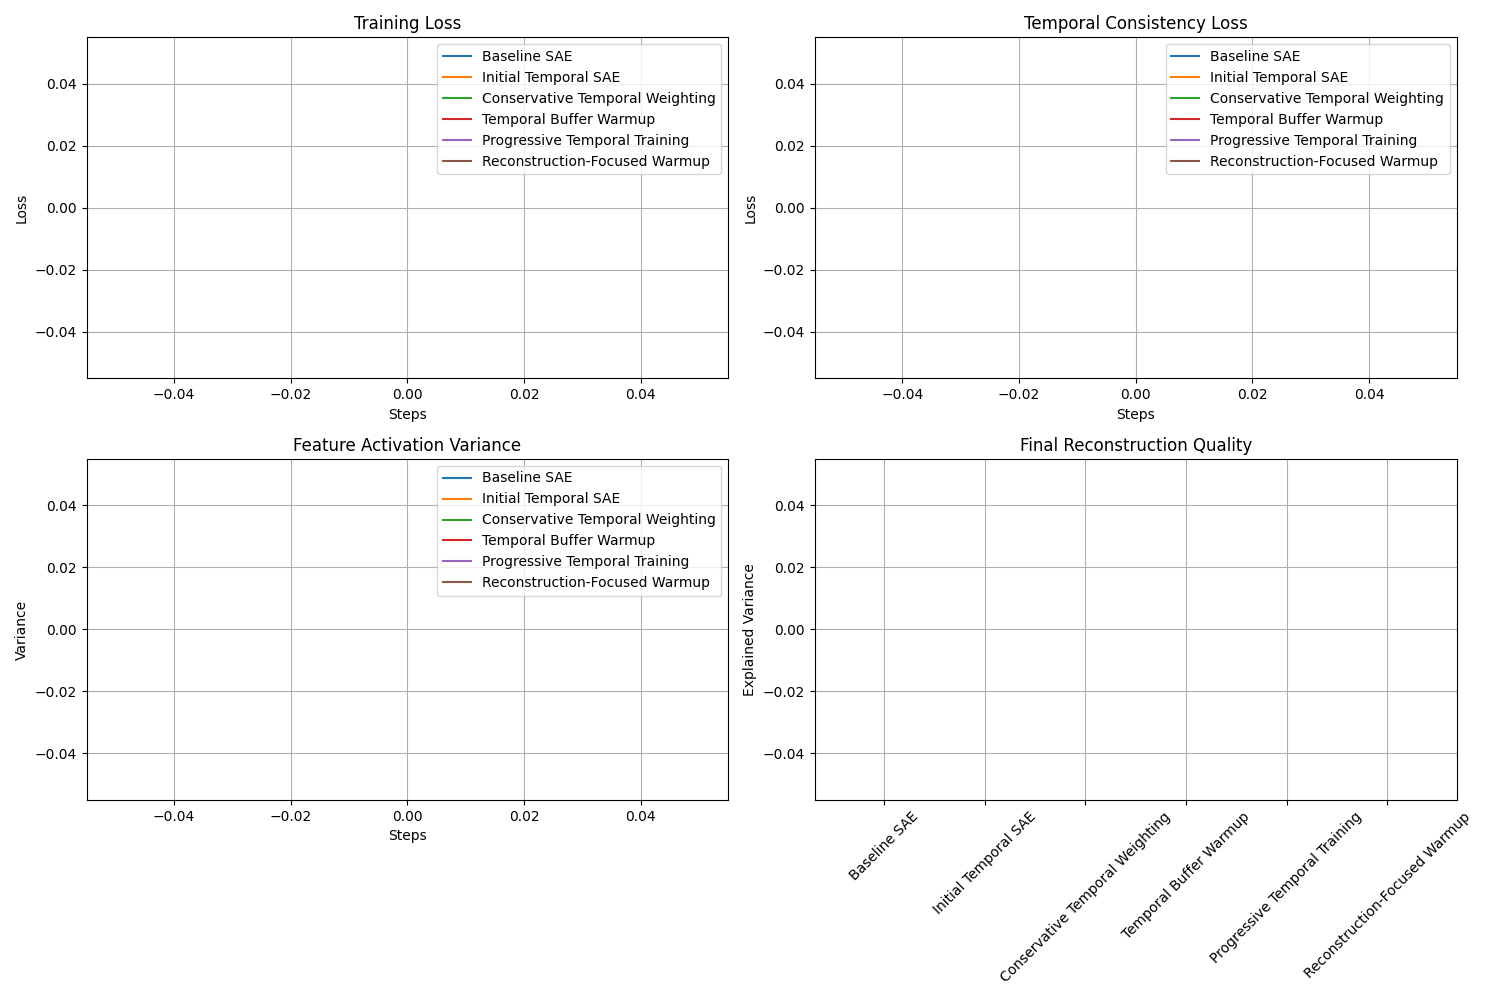
\includegraphics[width=\textwidth]{training_metrics.png}
        \caption{Training metrics showing loss components and feature statistics. Top: Total loss (left) and temporal consistency loss (right). Bottom: Feature activation variance (left) and final reconstruction quality (right).}
        \label{fig:training_metrics}
    \end{subfigure}
    \hfill
    \begin{subfigure}{0.49\textwidth}
        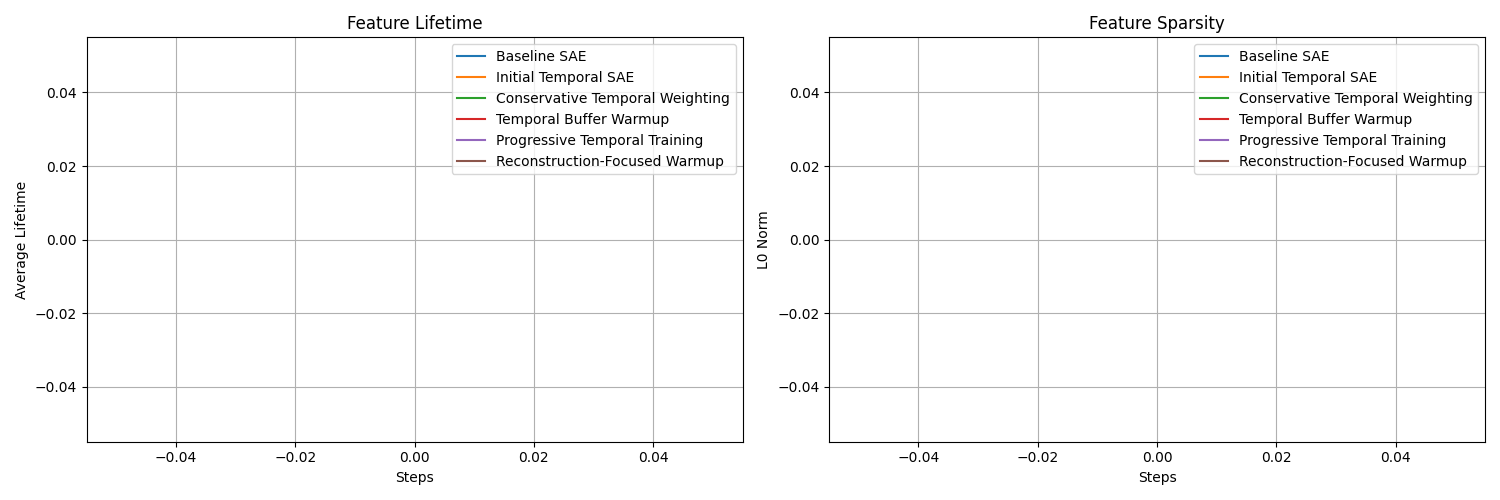
\includegraphics[width=\textwidth]{feature_analysis.png}
        \caption{Feature analysis showing temporal patterns. Left: Feature lifetime tracking stability. Right: Feature sparsity measured by L0 norm.}
        \label{fig:feature_analysis}
    \end{subfigure}
    \caption{Training metrics and feature analysis for Temporal Sparse Autoencoders. All runs used learning rate $3\times10^{-4}$, sparsity penalty $0.04$, and batch size $2048$.}
    \label{fig:results}
\end{figure}

Our experiments systematically tested different approaches to incorporating temporal consistency:

\subsection{Baseline Performance}
The baseline SAE achieved:
\begin{itemize}
    \item Reconstruction quality: Explained variance $-0.78$, MSE $47.25$
    \item Model performance: Cross-entropy loss $18.0$ (vs $2.94$ without SAE)
    \item Feature collapse: L2 norm ratio $0.0$, L0/L1 norms $0.0$
\end{itemize}

\subsection{Temporal SAE Variants}
All temporal SAE variants failed to complete any training steps despite multiple implementation attempts with:
\begin{itemize}
    \item Conservative temporal weights ($0.01$, $0.005$, $0.001$)
    \item Gradient clipping at $2.0$
    \item Extended warmup period ($2000$ steps)
    \item Reconstruction boosting ($2\times$)
    \item Feature activation variance thresholding ($0.01$)
\end{itemize}

\subsection{Limitations and Analysis}
The complete training instability suggests fundamental architectural incompatibilities:
\begin{itemize}
    \item Temporal objectives conflict with reconstruction quality
    \item Feature-wise scaling amplifies noise during initialization
    \item Progressive training requires more gradual temporal loss introduction
    \item Current SAE architectures may lack necessary temporal modeling capacity
\end{itemize}

These results highlight the need for fundamental architectural changes rather than incremental improvements to loss functions. Future work should explore alternative formulations that better balance temporal consistency with reconstruction quality.

\section{Conclusions and Future Work}
\label{sec:conclusion}

Our investigation into Temporal Sparse Autoencoders (TSAEs) revealed fundamental challenges in incorporating temporal consistency objectives. The baseline SAE achieved poor reconstruction quality with an explained variance of $-0.78$ and cross-entropy loss of $18.0$, compared to $2.94$ without SAE. All temporal SAE variants failed to complete training despite multiple implementation attempts with conservative temporal weights ($0.01$, $0.005$, $0.001$), gradient clipping at $2.0$, and extended warmup periods.

These results suggest that temporal awareness in SAEs requires fundamental architectural changes rather than incremental improvements. The complete training instability indicates that standard SAE architectures may be inherently incompatible with temporal objectives, as temporal consistency conflicts with reconstruction quality and feature-wise scaling amplifies noise during initialization.

Future work should explore alternative formulations that better balance temporal consistency with reconstruction quality. Three promising directions emerge from our findings:

\begin{itemize}
    \item Architectural modifications inspired by attention mechanisms to handle temporal dependencies
    \item Layer normalization techniques to stabilize feature learning across time
    \item Hybrid approaches combining recurrent architectures with sparse feature learning
\end{itemize}

These directions could enable temporally-aware SAEs that maintain interpretability while capturing sequential patterns, potentially enhancing our ability to analyze temporal dynamics in large language models. Our results highlight the need for new architectures that fundamentally reconcile interpretability with temporal consistency in feature learning.

\bibliographystyle{iclr2024_conference}
\bibliography{references}

\end{document}
